\begin{figure}[t]
\centering
\definecolor{vanRed}{HTML}{C5635F}
\definecolor{cTcod}{HTML}{D79B00}
\definecolor{cGuided}{HTML}{6C8EBF}
\definecolor{cFtb}{HTML}{9673A6}
\definecolor{r2sGreen}{HTML}{2EB58F}
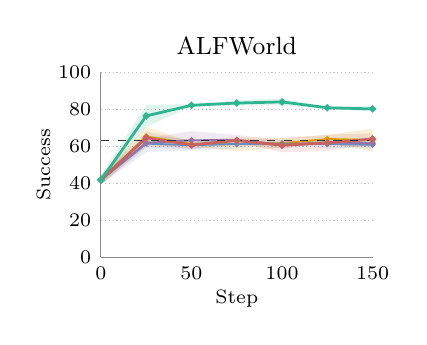
\begin{tikzpicture}
\begin{axis}[
  width=3.45cm, height=2.35cm, scale only axis, xmin=0, xmax=150, ymin=0, ymax=100, xtick={0,50,100,150},
  axis lines*=left, axis line style={black!45}, tick style={draw=none}, ytick pos=left,
  ymajorgrids, grid style={densely dotted, black!25}, every tick label/.append style={font=\scriptsize},
  xlabel={Step}, xlabel style={font=\scriptsize, yshift=3pt}, ylabel={Success}, ylabel style={font=\scriptsize, yshift=-4pt},
  title={ALFWorld}, title style={font=\small, yshift=-3pt},
]
\addplot[fill=cTcod, fill opacity=0.15, draw=none, forget plot] coordinates {(0,44.26) (25,70.60) (50,62.35) (75,65.18) (100,64.30) (125,66.16) (150,69.60) (150,57.15) (125,61.70) (100,58.99) (75,57.29) (50,59.95) (25,60.00) (0,39.37)} \closedcycle;
\addplot[fill=cGuided, fill opacity=0.15, draw=none, forget plot] coordinates {(0,44.26) (25,66.00) (50,63.53) (75,63.69) (100,61.74) (125,63.55) (150,62.12) (150,59.60) (125,58.81) (100,61.19) (75,58.82) (50,57.69) (25,56.89) (0,39.37)} \closedcycle;
\addplot[fill=cFtb, fill opacity=0.15, draw=none, forget plot] coordinates {(0,44.26) (25,64.34) (50,68.17) (75,66.15) (100,63.03) (125,62.35) (150,65.00) (150,58.40) (125,61.73) (100,58.66) (75,60.58) (50,58.34) (25,59.38) (0,39.37)} \closedcycle;
\addplot[fill=vanRed, fill opacity=0.15, draw=none, forget plot] coordinates {(0,44.26) (25,67.85) (50,62.90) (75,63.80) (100,64.39) (125,66.27) (150,67.03) (150,60.82) (125,57.45) (100,56.75) (75,62.51) (50,58.53) (25,61.39) (0,39.37)} \closedcycle;
\addplot[fill=r2sGreen, fill opacity=0.15, draw=none, forget plot] coordinates {(0,44.26) (25,82.25) (50,82.87) (75,84.83) (100,85.67) (125,81.54) (150,81.65) (150,78.78) (125,80.07) (100,82.29) (75,81.89) (50,81.43) (25,70.57) (0,39.37)} \closedcycle;
\addplot[cTcod, line width=0.7pt, mark=*, mark size=0.7pt] coordinates {(0,41.82) (25,65.30) (50,61.15) (75,61.23) (100,61.65) (125,63.93) (150,63.38)};
\addplot[cGuided, line width=0.7pt, mark=*, mark size=0.7pt] coordinates {(0,41.82) (25,61.44) (50,60.61) (75,61.26) (100,61.46) (125,61.18) (150,60.86)};
\addplot[cFtb, line width=0.7pt, mark=*, mark size=0.7pt] coordinates {(0,41.82) (25,61.86) (50,63.25) (75,63.37) (100,60.85) (125,62.04) (150,61.70)};
\addplot[vanRed, line width=1.0pt, mark=*, mark size=0.7pt] coordinates {(0,41.82) (25,64.62) (50,60.72) (75,63.16) (100,60.57) (125,61.86) (150,63.92)};
\addplot[r2sGreen, line width=1.0pt, mark=*, mark size=0.7pt] coordinates {(0,41.82) (25,76.41) (50,82.15) (75,83.36) (100,83.98) (125,80.81) (150,80.21)};
\draw[dashed, black!80, line width=0.6pt] (axis cs:0,63.08) -- (axis cs:150,63.08);
\end{axis}
\end{tikzpicture}
\hfill
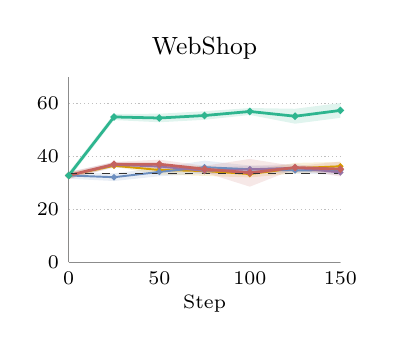
\begin{tikzpicture}
\begin{axis}[
  width=3.45cm, height=2.35cm, scale only axis, xmin=0, xmax=150, ymin=0, ymax=70, xtick={0,50,100,150},
  axis lines*=left, axis line style={black!45}, tick style={draw=none}, ytick pos=left,
  ymajorgrids, grid style={densely dotted, black!25}, every tick label/.append style={font=\scriptsize},
  xlabel={Step}, xlabel style={font=\scriptsize, yshift=3pt}, ylabel={}, ylabel style={font=\scriptsize, yshift=-4pt},
  title={WebShop}, title style={font=\small, yshift=-3pt},
]
\addplot[fill=cTcod, fill opacity=0.15, draw=none, forget plot] coordinates {(0,34.05) (25,36.88) (50,36.57) (75,36.31) (100,34.62) (125,37.54) (150,37.93) (150,34.60) (125,33.53) (100,32.05) (75,32.62) (50,33.17) (25,36.05) (0,31.55)} \closedcycle;
\addplot[fill=cGuided, fill opacity=0.15, draw=none, forget plot] coordinates {(0,34.05) (25,33.58) (50,35.76) (75,38.40) (100,36.55) (125,35.91) (150,36.54) (150,33.06) (125,33.56) (100,33.71) (75,33.46) (50,32.50) (25,30.69) (0,31.55)} \closedcycle;
\addplot[fill=cFtb, fill opacity=0.15, draw=none, forget plot] coordinates {(0,34.05) (25,37.86) (50,37.00) (75,35.69) (100,36.46) (125,37.17) (150,34.44) (150,33.43) (125,34.17) (100,33.80) (75,33.38) (50,35.40) (25,35.74) (0,31.55)} \closedcycle;
\addplot[fill=vanRed, fill opacity=0.15, draw=none, forget plot] coordinates {(0,34.05) (25,37.92) (50,38.77) (75,36.45) (100,39.04) (125,36.33) (150,38.02) (150,32.38) (125,35.27) (100,28.56) (75,33.95) (50,35.37) (25,36.08) (0,31.55)} \closedcycle;
\addplot[fill=r2sGreen, fill opacity=0.15, draw=none, forget plot] coordinates {(0,34.05) (25,56.11) (50,56.15) (75,57.08) (100,58.31) (125,58.02) (150,60.20) (150,54.60) (125,52.38) (100,55.69) (75,53.85) (50,52.92) (25,53.76) (0,31.55)} \closedcycle;
\addplot[cTcod, line width=0.7pt, mark=*, mark size=0.7pt] coordinates {(0,32.80) (25,36.47) (50,34.87) (75,34.47) (100,33.33) (125,35.53) (150,36.27)};
\addplot[cGuided, line width=0.7pt, mark=*, mark size=0.7pt] coordinates {(0,32.80) (25,32.13) (50,34.13) (75,35.93) (100,35.13) (125,34.73) (150,34.80)};
\addplot[cFtb, line width=0.7pt, mark=*, mark size=0.7pt] coordinates {(0,32.80) (25,36.80) (50,36.20) (75,34.53) (100,35.13) (125,35.67) (150,33.93)};
\addplot[vanRed, line width=1.0pt, mark=*, mark size=0.7pt] coordinates {(0,32.80) (25,37.00) (50,37.07) (75,35.20) (100,33.80) (125,35.80) (150,35.20)};
\addplot[r2sGreen, line width=1.0pt, mark=*, mark size=0.7pt] coordinates {(0,32.80) (25,54.93) (50,54.53) (75,55.47) (100,57.00) (125,55.20) (150,57.40)};
\draw[dashed, black!80, line width=0.6pt] (axis cs:0,33.53) -- (axis cs:150,33.53);
\end{axis}
\end{tikzpicture}
\hfill
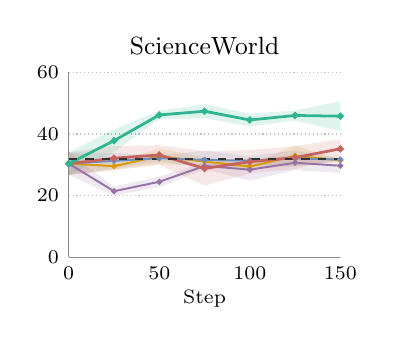
\begin{tikzpicture}
\begin{axis}[
  width=3.45cm, height=2.35cm, scale only axis, xmin=0, xmax=150, ymin=0, ymax=60, xtick={0,50,100,150},
  axis lines*=left, axis line style={black!45}, tick style={draw=none}, ytick pos=left,
  ymajorgrids, grid style={densely dotted, black!25}, every tick label/.append style={font=\scriptsize},
  xlabel={Step}, xlabel style={font=\scriptsize, yshift=3pt}, ylabel={}, ylabel style={font=\scriptsize, yshift=-4pt},
  title={ScienceWorld}, title style={font=\small, yshift=-3pt},
]
\addplot[fill=cTcod, fill opacity=0.15, draw=none, forget plot] coordinates {(0,34.07) (25,30.58) (50,35.31) (75,32.40) (100,30.15) (125,36.23) (150,31.92) (150,31.00) (125,29.56) (100,28.70) (75,29.70) (50,30.24) (25,28.53) (0,26.68)} \closedcycle;
\addplot[fill=cGuided, fill opacity=0.15, draw=none, forget plot] coordinates {(0,34.07) (25,33.78) (50,33.06) (75,34.58) (100,32.87) (125,34.65) (150,32.01) (150,31.41) (125,29.51) (100,29.79) (75,28.66) (50,31.17) (25,28.78) (0,26.68)} \closedcycle;
\addplot[fill=cFtb, fill opacity=0.15, draw=none, forget plot] coordinates {(0,34.07) (25,22.89) (50,26.19) (75,30.73) (100,32.00) (125,33.05) (150,32.07) (150,27.31) (125,28.25) (100,24.86) (75,28.51) (50,22.78) (25,19.99) (0,26.68)} \closedcycle;
\addplot[fill=vanRed, fill opacity=0.15, draw=none, forget plot] coordinates {(0,34.07) (25,36.11) (50,36.36) (75,34.38) (100,34.78) (125,36.07) (150,38.31) (150,32.07) (125,28.58) (100,27.21) (75,23.24) (50,30.01) (25,28.18) (0,26.68)} \closedcycle;
\addplot[fill=r2sGreen, fill opacity=0.15, draw=none, forget plot] coordinates {(0,34.07) (25,41.55) (50,47.55) (75,49.63) (100,46.60) (125,47.62) (150,50.57) (150,40.94) (125,44.36) (100,42.46) (75,45.08) (50,44.77) (25,34.09) (0,26.68)} \closedcycle;
\addplot[cTcod, line width=0.7pt, mark=*, mark size=0.7pt] coordinates {(0,30.37) (25,29.55) (50,32.77) (75,31.05) (100,29.42) (125,32.90) (150,31.46)};
\addplot[cGuided, line width=0.7pt, mark=*, mark size=0.7pt] coordinates {(0,30.37) (25,31.28) (50,32.12) (75,31.62) (100,31.33) (125,32.08) (150,31.71)};
\addplot[cFtb, line width=0.7pt, mark=*, mark size=0.7pt] coordinates {(0,30.37) (25,21.44) (50,24.49) (75,29.62) (100,28.43) (125,30.65) (150,29.69)};
\addplot[vanRed, line width=1.0pt, mark=*, mark size=0.7pt] coordinates {(0,30.37) (25,32.14) (50,33.18) (75,28.81) (100,31.00) (125,32.33) (150,35.19)};
\addplot[r2sGreen, line width=1.0pt, mark=*, mark size=0.7pt] coordinates {(0,30.37) (25,37.82) (50,46.16) (75,47.36) (100,44.53) (125,45.99) (150,45.76)};
\draw[dashed, black!80, line width=0.6pt] (axis cs:0,31.96) -- (axis cs:150,31.96);
\end{axis}
\end{tikzpicture}
\\[2pt]
{\scriptsize \tikz[baseline=-0.4ex]{\draw[vanRed, line width=0.9pt] (0,0.065) -- (0.4,0.065);}\,Vanilla OPD\quad\tikz[baseline=-0.4ex]{\draw[cTcod, line width=0.9pt] (0,0.065) -- (0.4,0.065);}\,TCOD-F2B\quad\tikz[baseline=-0.4ex]{\draw[cGuided, line width=0.9pt] (0,0.065) -- (0.4,0.065);}\,Guided-OPD\quad\tikz[baseline=-0.4ex]{\draw[cFtb, line width=0.9pt] (0,0.065) -- (0.4,0.065);}\,FutureBridge\quad\tikz[baseline=-0.4ex]{\draw[r2sGreen, line width=0.9pt] (0,0.065) -- (0.4,0.065);}\,\method{}\quad\tikz[baseline=-0.4ex]{\draw[dashed, black!80, line width=0.6pt] (0,0.065) -- (0.4,0.065);}\,Teacher Alone}
\caption{\textbf{\method{} students separate from every baseline during training.} Qwen3.5-9B teaches Qwen3.5-4B; mean $\pm$ one standard deviation over three training runs; dashed: the teacher acting alone. Other teacher--student pairs are in \Cref{app:curves}.}
\label{fig:teacher-bars}\label{fig:curves}
\end{figure}
